\printconcepts

\exercise{T/F: If $f(x,y)$ is differentiable on $S$, the $f$ is continuous on $S$.}{T}

\exercise{T/F: If $f_x$ and $f_y$ are continuous on $S$, then $f$ is differentiable on $S$.}{T}

\exercise{T/F: If $z=f(x,y)$ is differentiable, then the change in $z$ over small changes $\dd x$ and $\dd y$ in $x$ and $y$ is approximately $\dd z$.}{T}

\exercise{Finish the sentence: ``The new $z$-value is approximately the old $z$-value plus the approximate \underline{\hskip .5in}.''}{amount of change}

\printproblems

\begin{exerciseset}{In Exercises}{, find the total differential $\dd z$.}

\exercise{$z = x\sin y + x^2$}{$\dd z = (\sin y + 2x)\dd x + (x\cos y)\dd y$}

\exercise{$z = (2x^2+3y)^2$}{$\dd z = 8x(2x^2+3y)\dd x + 6(2x^2+3y)\dd y$}

\exercise{$z = 5x-7y$}{$\dd z = 5\dd x -7\dd y$}

\exercise{$z = xe^{x+y}$}{$\dd z = (e^{x+y}+xe^{x+y})\dd x +xe^{x+y}\dd y$}

\end{exerciseset}


\input{exercises/12-04-exset-02}

\exercisesetinstructions[Exercises]{ ask a variety of questions dealing with approximating error and sensitivity analysis.}

\exercise{A cylindrical storage tank is to be 2ft tall with a radius of 1ft. Is the volume of the tank more sensitive to changes in the radius or the height?}{The total differential of volume is $\dd V = 4\pi\dd r + \pi\dd h$. The coefficient of $\dd r$ is greater than the coefficient of $\dd h$, so the volume is more sensitive to changes in the radius.}

\exercise{\textbf{Projectile Motion:} The $x$-value of an object moving under the principles of projectile motion is $x(\theta,v_0,t)= (v_0\cos\theta)t$. A particular projectile is fired with an initial velocity of $v_0=250$ft/s and an angle of elevation of $\theta = 60^{\circ}$. It travels a distance of $375$ft in 3 seconds.\bigskip

Is the projectile more sensitive to errors in initial speed or angle of elevation?%
}{Distance of the projectile is a function of two variables (leaving $t=3$): $D(v_0,\theta) = 3v_0\cos\theta$. The total differential of $D$ is $\dd D = 3\cos\theta\dd v_0-3v_0\sin\theta\dd\theta$. The coefficient of $\dd\theta$ has a much greater magnitude than the coefficient of $\dd v_0$, so a small change in the angle of elevation has a much greater effect on distance traveled than a small change in initial velocity.}

\exercise{The length $\ell$ of a long wall is to be approximated. The angle $\theta$, as shown in the diagram (not to scale), is measured to be $85^{\circ}$, and the distance $x$ is measured to be 30'. Assume that the triangle formed is a right triangle.\bigskip

Is the measurement of the length of $\ell$ more sensitive to errors in the measurement of $x$ or in $\theta$?

\begin{minipage}{\linewidth}
\centering
\pdftooltip{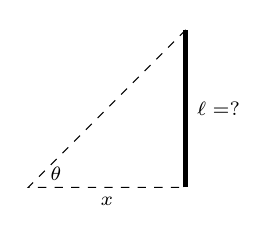
\begin{tikzpicture}
\draw [ultra thick] (1,-1) -- node [pos=.5,right] {\scriptsize $\ell=$?}(1,1);
\draw [dashed] (1,1) -- (-1,-1) node [xshift=10pt,yshift=5pt] {\scriptsize $\theta$} -- node [pos=.5,below] {\scriptsize $x$} (1,-1);
%\draw (-.5,0) -- node [pos=.5,draw=white,fill=white] {\scriptsize $50'$} (1,0);
\end{tikzpicture}}{ALT-TEXT-TO-BE-DETERMINED}
\end{minipage}%
}{Using trigonometry, $\ell = x\tan\theta$, so $\dd\ell = \tan\theta\dd x + x\sec^2\theta\dd\theta$. With $\theta = 85^{\circ}$ and $x=30$, we have $\dd\ell = 11.43\dd x+3949.38\dd\theta$. The measured length of the wall is much more sensitive to errors in $\theta$ than in $x$. While it can be difficult to compare sensitivities between measuring feet and measuring degrees (it is somewhat like ``comparing apples to oranges''), here the coefficients are so different that the result is clear: a small error in degree has a much greater impact than a small error in distance.}

\exercise{It is ``common sense'' that it is far better to measure a long distance with a long measuring tape rather than a short one. A measured distance $D$ can be viewed as the product of the length $\ell$ of a measuring tape times the number $n$ of times it was used. For instance, using a 3' tape 10 times gives a length of 30'. To measure the same distance with a 12' tape, we would use the tape 2.5 times. (I.e., $30=12\times 2.5$.) Thus $D = n\ell$.\bigskip

Suppose each time a measurement is taken with the tape, the recorded distance is within 1/16'' of the actual distance. (I.e., $d\ell = 1/16'' \approx 0.005$ft). Using differentials, show why common sense proves correct in that it is better to use a long tape to measure long distances.%
}{With $D = n\ell$, the total differential is $\dd D = \ell\dd n+ n\dd\ell.$ If one measures with a short tape, $n$ must be large and hence $n\dd\ell$ is going to be greater than when a large tape is used (wherein $n$ will be small).}

\exercisesetend


\exercisesetinstructions{, find the total differential $\dd w$.}

\exercise{$w= x^2yz^3$}{$\dd w = 2xyz^3\dd x + x^2z^3\dd y + 3x^2yz^2\dd z$}

\exercise{$w= e^x\sin y\ln z$}{$\dd w = e^x\sin y\ln z\dd x + e^x\cos y\ln z\dd y + e^x\sin y\frac1z\dd z$}

\exercisesetend


\begin{exerciseset}{In Exercises}{, use the information provided and the total differential to make the given approximation.}

\exercise{$f(3,1) = 7$,\ \  $f_x(3,1) = 9$, \ \ $f_y(3,1) = -2$.  Approximate $f(3.05, 0.9)$.}{$\dd x = 0.05$, $\dd y = -0.1$. $\dd z = 9(.05)+(-2)(-0.1) = 0.65$. So $f(3.05,0.9) \approx 7+0.65=7.65$.}

\exercise{$f(-4,2) = 13$,\ \  $f_x(-4,2) = 2.6$, \ \ $f_y(-4,2) = 5.1$.  Approximate $f(-4.12, 2.07)$. }{$\dd x = -0.12$, $\dd y = 0.07$. $\dd z = 2.6(-.12)+(5.1)(0.07) = 0.045$. So $f(-4.12, 2.07) \approx 13+0.045=13.045$.}

\exercise{$f(2,4,5) = -1$,\ \ $f_x(2,4,5) = 2$,\ \ $f_y(2,4,5) = -3$,\ \ $f_z(2,4,5) = 3.7$. Approximate $f(2.5,4.1,4.8)$.}{$\dd x = 0.5$, $\dd y = 0.1$, $\dd z = -0.2$.\\
$\dd w = 2(0.5) + (-3)(0.1) + 3.7(-0.2) = -0.04$, so $f(2.5, 4.1, 4.8) \approx -1-0.04 = -1.04$.}

\exercise{$f(3,3,3) = 5$,\ \ $f_x(3,3,3) = 2$,\ \ $f_y(3,3,3) = 0$,\ \ $f_z(3,3,3) = -2$. Approximate $f(3.1, 3.1,3.1)$.}{$\dd x = 0.1$, $\dd y = 0.1$, $\dd z = 0.1$.\\
$\dd w = 2(0.1) + (0)(0.1) + (-2)(.1) = 0$, so $f(3.1,3.1,3.1) \approx 5+0=5$.}

\end{exerciseset}


\exercise{Find where the function $z=\sqrt{x^2+y^2}$ is differentiable.}{Everywhere except the origin.}

% todo add exercises asking where a function is differentiable
